% REMEMBER: Write the thesis from the view of the reader. How would I like to READ the thesis?

\chapter{Background}%
\label{cha:background}

\mnote{input generation also explained}
This chapter will give some background about how Scratch works and why testing Scratch programs is a difficult task.
It will also highlight some related work, which has tackled to problem of testing Scratch programs.

\section{Scratch}%
\label{sec:scratch}
% No extensions
% Block-based code eliminates the possibility of syntax errors and makes programming more intuitive by letting the user pick blocks from a drawer of pre-defined blocks instead of having the user memorize a programming language's keywords.
% Scratch heavily focuses on multimedia, as graphics and audio can easily be integrated into Scratch projects.
% Whenever a sprite is cloned, it runs all of its scripts, which have a ''when I start as a clone'' hat.

\mnote{TODO: Scratch is run and developed inside a GUI, run with a VM}

\begin{wrapfigure}{r}{0.35\textwidth + 5mm}
    \vspace{-3mm}
    \centering
    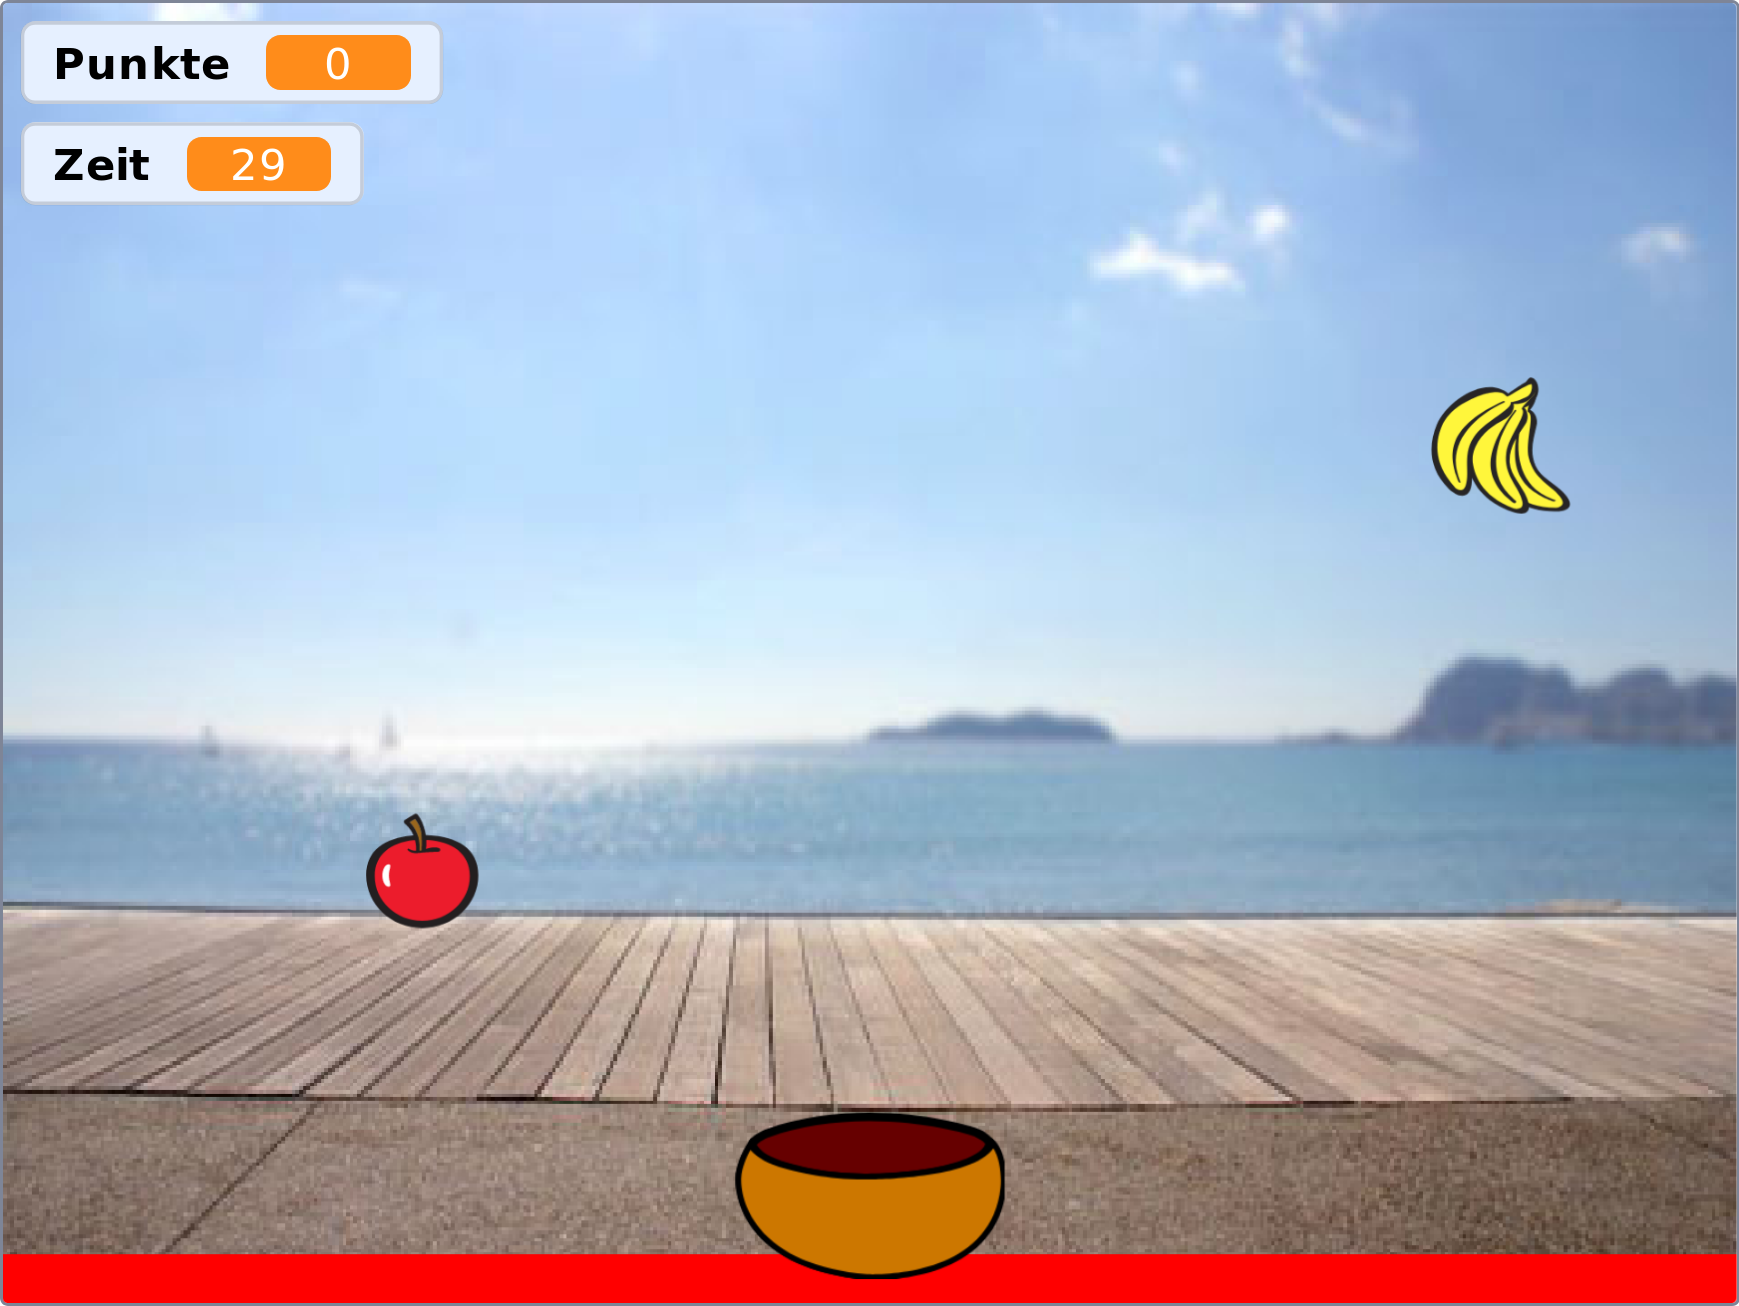
\includegraphics[width=0.35\textwidth]{scratch-stage}
    \caption{A catching game implemented in Scratch}
    \label{fig:a_catching_game_implemented_in_scratch}
    \vspace{-3mm}
\end{wrapfigure}

Scratch is a programming language developed by the MIT Media Lab~\cite{scratch}.
Its main goal is to offer an intuitive programming language suited for programming novices and children.
It implements a block-based code system, which eliminates the possibility of syntax errors,
and allows users to easily integrate graphics and audio into their program.

\begin{wrapfigure}{r}{0.45\textwidth + 5mm}
    \vspace{-3mm}
    \centering
    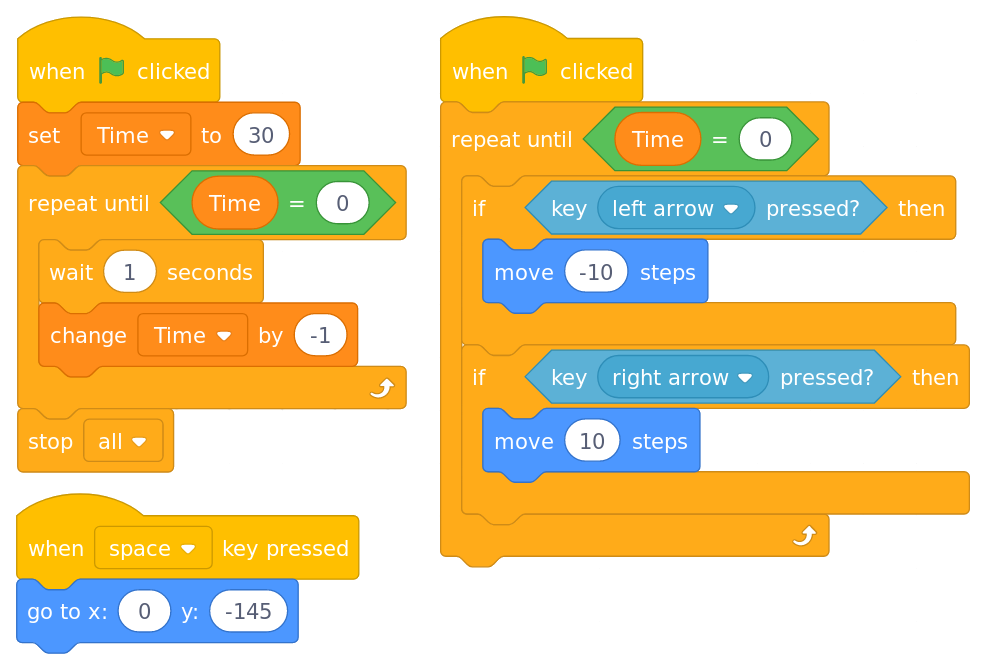
\includegraphics[width=0.45\textwidth]{scratch-code}
    \caption{Scratch blocks}
    \label{fig:scratch_blocks}
    \vspace{-3mm}
\end{wrapfigure}

\textbf{Input and output.}
Scratch programs create interactive two-dimensional animations through a number of visual objects (the \textit{sprites}) on a background (the \textit{stage}).
The program manipulates sprites' appearance, position, size, rotation, visual effects and sounds.
Furthermore, Sprites can also display messages and ask the user to type answers into a text box.
Programs can react to user input like keyboard key presses, mouse clicks or mouse cursor movement.

\textbf{Code.}
Programming in Scratch is done by sticking together a structure of pre-defined blocks.
Multiple blocks are combined together with a \textit{hat} to make up a \textit{script}.
Scripts are called through a event, which is defined by their hat. % TODO show hat, code, script region in figure
There are a variety of different events in Scratch.
The main event is the \textit{green flag}, which is the entry point of the program.
This event is emitted when the user starts the program by pressing the start button.
The program then starts by executing all scripts, which are equipped with a ''when green flag is pressed'' hat.
Other events include key presses on the keyboard, clicks on a specific sprite, and events sent from different scripts.
Active scripts effectively run in parallel until the end of each script is reached, or until the script is stopped by itself or another script.

\textbf{Sprite and variables.}
Each sprite contains its own code and variables.
These variables, as well as the sprite itself can only be manipulated by the sprite's own scripts.
The only exception to this rule is the stage, whose variables are accessible by all other sprites as well.
Sprites can interact with each other through a messaging system and through the stage's variables.
By \textit{cloning} sprites, the program can create multiple instances of a sprite, which behave alike.
The cloned sprites then also share the original sprite's variables.

\begin{wrapfigure}{r}{0.45\textwidth + 5mm}
    \centering
    \vspace{-4mm}
    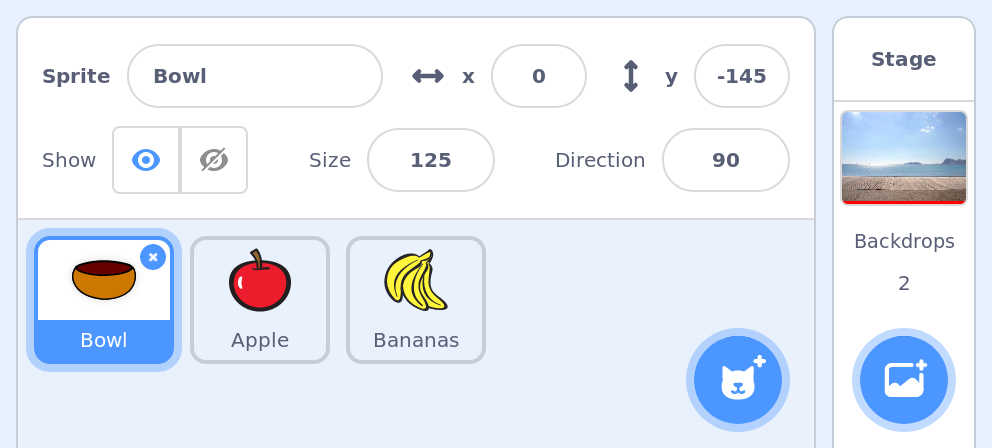
\includegraphics[width=0.45\textwidth]{scratch-sprites}
    \caption{The sprite menu}
    \label{fig:the_sprite_menu}
\end{wrapfigure}

\section{Previous Testing Approaches}%
\label{sec:previous_testing_approaches}

Although automatic assessment of Scratch programs is still an open problem,
at least two other projects have tackled this task through different approaches.

\textbf{Hairball.}
Boe et al. developed Hairball~\cite{hairball} to perform static analysis on Scratch programs.
Hairball is implemented as a standalone Python program.
It allows users to load a saved project file and analyze it by iterating through its blocks.
% Example applications of Hairball are detecting code smells or finding out if a desired programming concept is implemented in the program.
A example application is the web-based assessment tool called Dr. Scratch~\cite{drscratch} by Jes\'{u}s et al..
Dr. Scratch uses Hairball to measure the complexity of uploaded Scratch programs in various categories and scores them accordingly.
Though Hairball is very useful for analyzing programs statically, it is not fitted to test the functionality and the correctness of a program.
To do this, a dynamic testing approach is more suitable.

\textbf{ITCH.}
ITCH (Individual Testing of Computer Homework for Scratch Assignments)~\cite{itch} by David E. Johnson is another Scratch assessment tool.
Like Hairball, it is also implemented in Python.
But it follows an entirely different approach.
ITCH performs dynamic testing by reducing the Scratch programs to simple textual input and output operations.
Scratch supports these operations through "ask" and "say" blocks.
To automate the input and output, "ask" and "say" blocks are replaced with structures, which give the program configured input text, and save the result to the project file.
ITCH then executes the program, saves it, and analyzes the saved project file to generate a test report.
This allows simple input-output-testing for Scratch, which is useful for testing the correctness of an implemented algorithm.
But ITCH has a major drawback: Reducing Scratch programs to textual IO means that only a small subset of Scratch's functionality is available to the programs under test.
Sprite manipulation and such cannot be tested with ITCH.
In this case, programming environments like BlockPy~\cite{blockpy} are probably a better choice that Scratch,
since they allow to translate the block-based code into a traditional programming language (in this case: Python).

% \section{Black Box Testing}
%
% - Black box approach:
%     - Block box testing bases tests on the specification of the tested program
%     - Tests are written without knowledge of the internals of a program
%     - Program is seen as a ''black box'' that takes some input and produces some output.
%     - Program specification is in the case of Scratch programs most likely a task description for some course or tutorial
%
%     - Input for the black box is user interaction through mouse and keyboard
%     - Interact only how a user can interact with the program
%         - Since Scratch can only be controlled through user interaction and has no API to call blocks or scripts,
%           it only makes sense to control the program this way in the test
%         - No information about the internals of the program other than sprite and variable names
%             - Sprite names should be included in the specification so the test can more easily identify sprites
%             - Giving no or little information about the implementation makes sense for a task description
%     - Output of the black box are changes on Scratch's stage
%     - Test only what the user sees
%         - Only information about sprites and variables (both can be shown on screen)
%         - Sprite positions, movement, looks, etc.
%
% \section{Automatic Test Generation}%
% \label{sec:automatic_test_generation}

\section{Challenges of Testing Scratch Programs}

Dynamically testing Scratch programs is not a straightforward task.
There exist multiple challenges that have to be overcome in order to test Scratch programs accurately.
This section explains these challenges and how the presented approach overcomes these challenges.

\textbf{Parallel scripts.}
One problem is Scratch's code system.
It does not have a traditional mechanism to structure code into methods, which return values.
Furthermore, scripts run in parallel and may depend on one another.
This makes it hard to test a part of the program in isolation from the rest of the program.
One could circumvent this problem by restricting the tested programs, like ITCH~\cite{itch} does it,
but this defeats the purpose of using Scratch as a language.
% To deal with this challenge, this work proposes a black-box testing approach.
% This way, the test code does not have to concern itself with the internals of the program.
% Scratch programs can be controlled by simulating user input, instead of calling specific scripts.
% Tests can then check the visual and auditory output of the program.

\textbf{GUI input and output.}
Scratch is entirely run inside a GUI interface and therefore lacks traditional IO mechanisms.
Its output consists of visual animations and audio, which difficult hard to analyze automatically.
Likewise, Scratch's input, which mainly consists of keyboard and mouse input, can make interacting with the program problematic.
% We are going to deal with this problem by creating a wrapper around Scratch,
% which can be used to simulate input and access information about the sprites which make up the output.
% Tests can then use methods, which the wrapper provides, instead of manually interacting with the Scratch program.

\begin{wrapfigure}{r}{0.25\textwidth + 5mm}
    \centering
    \vspace{-6mm}
    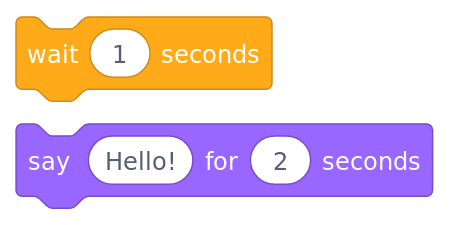
\includegraphics[width=0.25\textwidth]{code-timing}
    \vspace{-3mm}
    \caption{Delaying blocks}
    \label{fig:delaying_blocks}
\end{wrapfigure}

\textbf{Absolute timings.}
Scratch offers code blocks to delay the execution of a script, which often find use in typical game-like programs.
These blocks use absolute timings to implement the delay.
Basically, they save the current time when they pause the script,
then later resume the execution of the script when the difference between the current time and the saved time reached the desired delay length.
This means that the execution of the Scratch program can only be paused or delayed for a very short time without interfering with these timings.
Pausing the execution of the Scratch program for too long, while a delay is active,
takes away execution time from other scripts, which are executed parallel to the delay.
This can potentially have an impact on the program under test.
% Therefore, additional computations by the testing procedure must be fast enough to avoid interfering with the program under test.
\mnote{Reference the evaluation section about timings here?}

% === Many tested properties will depend on time
% - A tested property might depend on a previous value
%     - e.g. check if a sprite is moving right
%     - sprites save the values from the previous execution step
% - Some tested properties should hold for a time or for the whole execution
%     - Provide a way to define constraints that must always hold
